\documentclass[12pt,a4paper]{article}

\usepackage[a4paper,margin=1in]{geometry}
\usepackage{graphicx}
\usepackage{float}
\usepackage{booktabs}
\usepackage{array}
\usepackage{hyperref}
\usepackage{titlesec}
\usepackage{setspace}
\usepackage{fancyhdr}
\usepackage{xcolor}
\usepackage{caption}
\usepackage{tikz}
\usetikzlibrary{calc}

\setstretch{1.25}

\pagestyle{fancy}
\fancyhf{}
\rhead{Digital Clock Project}
\lhead{Embedded Systems}
\cfoot{\thepage}

\hypersetup{
colorlinks=true,
linkcolor=blue,
urlcolor=blue
}

\begin{document}

%%%%%%%%%%%%%%%%%%%%%%%%%%%%%%%%%%%%%%%%%%%%%%%%%%
% TITLE PAGE
%%%%%%%%%%%%%%%%%%%%%%%%%%%%%%%%%%%%%%%%%%%%%%%%%%

\begin{titlepage}

\begin{tikzpicture}[remember picture,overlay]
\draw[line width=2pt]
($(current page.north west)+(1cm,-1cm)$)
rectangle
($(current page.south east)+(-1cm,1cm)$);
\end{tikzpicture}

\centering

\vspace*{1.8cm}

{\Huge\bfseries DIGITAL CLOCK\\[0.4cm]}

{\Large Using ATmega328P Microcontroller}

\vspace{1.5cm}

{\Large\bfseries Project Report}

\vspace{1.8cm}

\begin{tabular}{ll}
\textbf{Microcontroller} & ATmega328P-PU\\
\textbf{Display} & 4-Digit Seven Segment Display\\
\textbf{Clock Source} & 16 MHz Crystal Oscillator\\
\textbf{Power Supply} & 5V USB Supply\\
\textbf{Programming} & Arduino IDE (Embedded C)\\
\textbf{Assembly} & Perfboard Soldering\\
\textbf{CAD Software} & Fusion 360\\
\textbf{Enclosure} & Custom Designed and 3D Printed\\
\end{tabular}

\vfill

\textbf{\Large Submitted By}

\vspace{0.4cm}

Kalpana Kumari

June, 2026

\end{titlepage}

%%%%%%%%%%%%%%%%%%%%%%%%%%%%%%%%%%%%%%%%%%%%%%%%%%
% CONTENTS
%%%%%%%%%%%%%%%%%%%%%%%%%%%%%%%%%%%%%%%%%%%%%%%%%%

\tableofcontents

\newpage

%%%%%%%%%%%%%%%%%%%%%%%%%%%%%%%%%%%%%%%%%%%%%%%%%%
% INTRODUCTION
%%%%%%%%%%%%%%%%%%%%%%%%%%%%%%%%%%%%%%%%%%%%%%%%%%

\section{Introduction}

A digital clock is an embedded electronic system that displays the current time in a numerical format using seven-segment displays. Unlike conventional analog clocks, a digital clock performs continuous time calculations through a programmable microcontroller while refreshing the display at a sufficiently high speed to provide a stable visual output.

The objective of this project was not only to build a working digital clock but also to understand the complete hardware development cycle of an embedded system. The project began with an Arduino Uno based prototype to verify the circuit and firmware. After successful testing, the Arduino board was replaced by a standalone ATmega328P microcontroller, making the circuit compact and independent.

The complete circuit was then assembled permanently on a perfboard through soldering. Finally, a custom enclosure was designed using CAD software and manufactured using a 3D printer, giving the project a professional appearance while protecting the internal electronics.

The project demonstrates the integration of electronics, embedded programming, PCB assembly, CAD modelling and additive manufacturing into a single functional product.

%%%%%%%%%%%%%%%%%%%%%%%%%%%%%%%%%%%%%%%%%%%%%%%%%%
% OBJECTIVES
%%%%%%%%%%%%%%%%%%%%%%%%%%%%%%%%%%%%%%%%%%%%%%%%%%

\section{Objectives}

The major objectives of this project are listed below:

\begin{itemize}

\item To design and implement a standalone digital clock using the ATmega328P microcontroller.

\item To understand multiplexing techniques used for driving a four-digit seven-segment display.

\item To develop firmware for accurate time counting using the Arduino IDE.

\item To interface push buttons for hour and minute adjustment.

\item To convert a breadboard prototype into a permanent soldered circuit.

\item To design a custom enclosure using Fusion 360.

\item To fabricate the enclosure using a 3D printer and assemble the final hardware.

\end{itemize}

%%%%%%%%%%%%%%%%%%%%%%%%%%%%%%%%%%%%%%%%%%%%%%%%%%
% PROJECT SPECIFICATIONS
%%%%%%%%%%%%%%%%%%%%%%%%%%%%%%%%%%%%%%%%%%%%%%%%%%

\section{Project Specifications}

\begin{table}[H]

\centering

\caption{Technical Specifications}

\begin{tabular}{|p{6cm}|p{7cm}|}

\hline

\textbf{Parameter} & \textbf{Specification}\\

\hline

Microcontroller & ATmega328P-PU\\

\hline

Operating Voltage & 5 V DC\\

\hline

Clock Frequency & 16 MHz Crystal Oscillator\\

\hline

Display Type & Four Digit Seven Segment Display\\

\hline

Programming Software & Arduino IDE\\

\hline

Programming Language & Embedded C (Arduino)\\

\hline

Input Controls & Three Push Buttons\\

\hline

Output Display & Hours and Minutes\\

\hline

Assembly Method & Perfboard Soldering\\

\hline

Enclosure Design & Fusion 360\\

\hline

Manufacturing Method & 3D Printing (PLA)\\

\hline

\end{tabular}

\end{table}

%%%%%%%%%%%%%%%%%%%%%%%%%%%%%%%%%%%%%%%%%%%%%%%%%%
% COMPONENTS
%%%%%%%%%%%%%%%%%%%%%%%%%%%%%%%%%%%%%%%%%%%%%%%%%%

\section{Components Required}

The following electronic components were used during the development of the project.

\begin{table}[H]

\centering

\caption{List of Components}

\begin{tabular}{|p{7cm}|c|}

\hline

\textbf{Component} & \textbf{Quantity}\\

\hline

ATmega328P Microcontroller & 1\\

\hline

4-Digit Seven Segment Display & 1\\

\hline

16 MHz Crystal Oscillator & 1\\

\hline

22 pF Capacitors & 2\\

\hline

100 nF Capacitors & 2\\

\hline

330 $\Omega$ Resistors & 9\\

\hline

10 k$\Omega$ Resistor & 1\\

\hline

Push Buttons & 3\\

\hline

Perfboard & 1\\

\hline

USB Power Module & 1\\

\hline

Connecting Wires & As Required\\

\hline

3D Printed Enclosure & 1\\

\hline

\end{tabular}

\end{table}

%%%%%%%%%%%%%%%%%%%%%%%%%%%%%%%%%%%%%%%%%%%%%%%%%%
% FEATURES
%%%%%%%%%%%%%%%%%%%%%%%%%%%%%%%%%%%%%%%%%%%%%%%%%%

\section{Features of the Digital Clock}

The developed digital clock provides the following features.

\begin{itemize}

\item Accurate time keeping using a 16 MHz crystal oscillator.

\item Four-digit multiplexed seven-segment display.

\item Independent standalone operation using ATmega328P.

\item Manual hour and minute adjustment through push buttons.

\item Compact permanent perfboard implementation.

\item Custom designed Fusion 360 enclosure.

\item Fully assembled 3D printed casing.

\item Low power operation through a standard 5 V USB supply.

\end{itemize}

%%%%%%%%%%%%%%%%%%%%%%%%%%%%%%%%%%%%%%%%%%%%%%%%%%
% WORKING PRINCIPLE
%%%%%%%%%%%%%%%%%%%%%%%%%%%%%%%%%%%%%%%%%%%%%%%%%%

\section{Working Principle}

The complete system operates using the ATmega328P microcontroller as the central processing unit.

The 16 MHz crystal oscillator generates a precise clock signal which allows the internal timers of the microcontroller to calculate one-second intervals accurately. The firmware continuously updates the stored values of hours and minutes based on these timer interrupts.

Since a four-digit seven-segment display contains many LEDs, multiplexing is employed to reduce the number of required I/O pins. The microcontroller rapidly activates one display digit at a time while simultaneously transmitting the appropriate segment data. Due to persistence of vision, all four digits appear illuminated continuously.

Three push buttons are provided for user interaction. Two buttons increment the hour and minute values respectively, while the third button is used to start or reset the clock depending on the programmed functionality.

After validating the circuit on a breadboard, the Arduino development board was replaced by the standalone ATmega328P microcontroller. The complete hardware was soldered on a perfboard and enclosed inside a custom-designed 3D printed casing to obtain a durable and compact final product.

\newpage
%%%%%%%%%%%%%%%%%%%%%%%%%%%%%%%%%%%%%%%%%%%%%%%%%%
% BREADBOARD PROTOTYPE
%%%%%%%%%%%%%%%%%%%%%%%%%%%%%%%%%%%%%%%%%%%%%%%%%%

\section{Breadboard Prototype}

Before constructing the final hardware, the complete circuit was first assembled on a breadboard using an Arduino Uno. This stage was carried out to verify all electrical connections, test the firmware, and ensure that the clock functioned correctly before making the circuit permanent.

The prototype allowed easy modification of the wiring and simplified debugging of hardware and software errors. Once the clock displayed the correct time and all push buttons functioned as expected, the design was finalized for standalone implementation.

\begin{figure}[H]
    \centering
    \includegraphics[width=0.75\textwidth]{breadboard.jpeg}
    \caption{Breadboard Prototype of the Digital Clock}
\end{figure}

%%%%%%%%%%%%%%%%%%%%%%%%%%%%%%%%%%%%%%%%%%%%%%%%%%
% CIRCUIT CONNECTIONS
%%%%%%%%%%%%%%%%%%%%%%%%%%%%%%%%%%%%%%%%%%%%%%%%%%

\section{Circuit Connections}

The digital clock consists of a microcontroller, a four-digit seven-segment display, three push buttons, crystal oscillator circuitry and supporting passive components. The major hardware connections are summarized below.

\begin{itemize}

\item Arduino digital pins D2--D8 are connected to display segments A--G through 330 $\Omega$ current limiting resistors.

\item Arduino pins D9--D12 are connected directly to the four digit enable pins for multiplexing.

\item Three push buttons are connected to analog pins A0, A1 and A2 for hour adjustment, minute adjustment and clock control respectively.

\item A 16 MHz crystal oscillator along with two 22 pF capacitors provides accurate timing for the ATmega328P.

\item A 10 k$\Omega$ resistor is connected to the RESET pin as a pull-up resistor.

\item Two 100 nF bypass capacitors are placed across the supply pins to improve power stability.

\end{itemize}

%%%%%%%%%%%%%%%%%%%%%%%%%%%%%%%%%%%%%%%%%%%%%%%%%%
% PIN MAPPING
%%%%%%%%%%%%%%%%%%%%%%%%%%%%%%%%%%%%%%%%%%%%%%%%%%

\section{Pin Mapping}

\begin{table}[H]

\centering

\caption{Microcontroller Pin Mapping}

\begin{tabular}{|c|l|}

\hline

\textbf{Arduino Pin} & \textbf{Function}\\

\hline

D2--D8 & Seven Segment Segments A--G\\

\hline

D9 & Digit 1 Select\\

\hline

D10 & Digit 2 Select\\

\hline

D11 & Digit 3 Select\\

\hline

D12 & Digit 4 Select\\

\hline

A0 & Hour Button\\

\hline

A1 & Minute Button\\

\hline

A2 & Start / Reset Button\\

\hline

5V & Power Supply\\

\hline

GND & Ground\\

\hline

\end{tabular}

\end{table}

%%%%%%%%%%%%%%%%%%%%%%%%%%%%%%%%%%%%%%%%%%%%%%%%%%
% STANDALONE IMPLEMENTATION
%%%%%%%%%%%%%%%%%%%%%%%%%%%%%%%%%%%%%%%%%%%%%%%%%%

\section{Standalone ATmega328P Implementation}

Once the breadboard prototype was successfully tested, the Arduino development board was removed and replaced with a standalone ATmega328P microcontroller.

To enable standalone operation, the ATmega328P was first programmed with the Arduino bootloader using the Arduino Uno configured as an ISP programmer. After the bootloader was successfully written, the microcontroller was capable of executing the clock firmware independently.

The standalone circuit required only a few external components including a 16 MHz crystal oscillator, two 22 pF capacitors, a pull-up resistor on the RESET pin, and proper power supply decoupling capacitors. This significantly reduced the circuit size while maintaining the same functionality as the Arduino prototype.

%%%%%%%%%%%%%%%%%%%%%%%%%%%%%%%%%%%%%%%%%%%%%%%%%%
% PROGRAMMING PROCESS
%%%%%%%%%%%%%%%%%%%%%%%%%%%%%%%%%%%%%%%%%%%%%%%%%%

\section{Programming Process}

The firmware for the digital clock was developed using the Arduino IDE. The program continuously updates the time using the internal timer of the ATmega328P while simultaneously refreshing the multiplexed display.

The following steps were followed during programming:

\begin{enumerate}

\item Configure the Arduino Uno as an ISP programmer.

\item Burn the bootloader onto the ATmega328P.

\item Develop and verify the digital clock firmware.

\item Upload the firmware using the ISP programmer.

\item Test the standalone circuit.

\item Verify proper display multiplexing and button operation.

\item Transfer the finalized circuit onto the perfboard.

\end{enumerate}

%%%%%%%%%%%%%%%%%%%%%%%%%%%%%%%%%%%%%%%%%%%%%%%%%%
% PROGRAM FLOW
%%%%%%%%%%%%%%%%%%%%%%%%%%%%%%%%%%%%%%%%%%%%%%%%%%

\section{Program Flow}

The software executed by the ATmega328P continuously performs the following operations.

\begin{enumerate}

\item Initialize all GPIO pins.

\item Configure timers for one-second intervals.

\item Read the state of the push buttons.

\item Update hours and minutes whenever a button is pressed.

\item Refresh the four-digit seven-segment display using multiplexing.

\item Repeat the process indefinitely.

\end{enumerate}

%%%%%%%%%%%%%%%%%%%%%%%%%%%%%%%%%%%%%%%%%%%%%%%%%%
% PERFBOARD ASSEMBLY
%%%%%%%%%%%%%%%%%%%%%%%%%%%%%%%%%%%%%%%%%%%%%%%%%%

\section{Permanent Perfboard Assembly}

After successful verification on the breadboard, the complete circuit was transferred onto a perforated circuit board (perfboard) to obtain a permanent and reliable implementation.

The ATmega328P was mounted on a 28-pin IC socket to facilitate replacement whenever required. All passive components, including resistors, capacitors, crystal oscillator and push buttons, were positioned carefully to minimize wiring complexity and improve maintainability.

During soldering, each connection was verified using a continuity test to eliminate short circuits and loose joints. Proper routing of jumper wires on the rear side of the board ensured a compact and organized layout.

\begin{figure}[H]
\centering
\includegraphics[width=0.8\textwidth]{front.jpg.jpeg}
\caption{Front View of the Soldered Perfboard}
\end{figure}

\begin{figure}[H]
\centering
\includegraphics[width=0.8\textwidth]{back.jpeg}
\caption{Rear View Showing Solder Connections}
\end{figure}

%%%%%%%%%%%%%%%%%%%%%%%%%%%%%%%%%%%%%%%%%%%%%%%%%%
% CAD DESIGN
%%%%%%%%%%%%%%%%%%%%%%%%%%%%%%%%%%%%%%%%%%%%%%%%%%

\section{3D CAD Design}

To provide mechanical protection and improve the overall appearance of the project, a custom enclosure was designed using Fusion 360.

The enclosure was divided into two separate components: a top lid and a bottom casing. The front panel contains openings for the four-digit seven-segment display and the three push buttons. Additional clearance was provided for the USB power connector to ensure easy accessibility.

The dimensions of the enclosure were determined according to the overall size of the perfboard, allowing sufficient clearance for all electronic components while maintaining a compact form factor.

\begin{figure}[H]
    \centering

    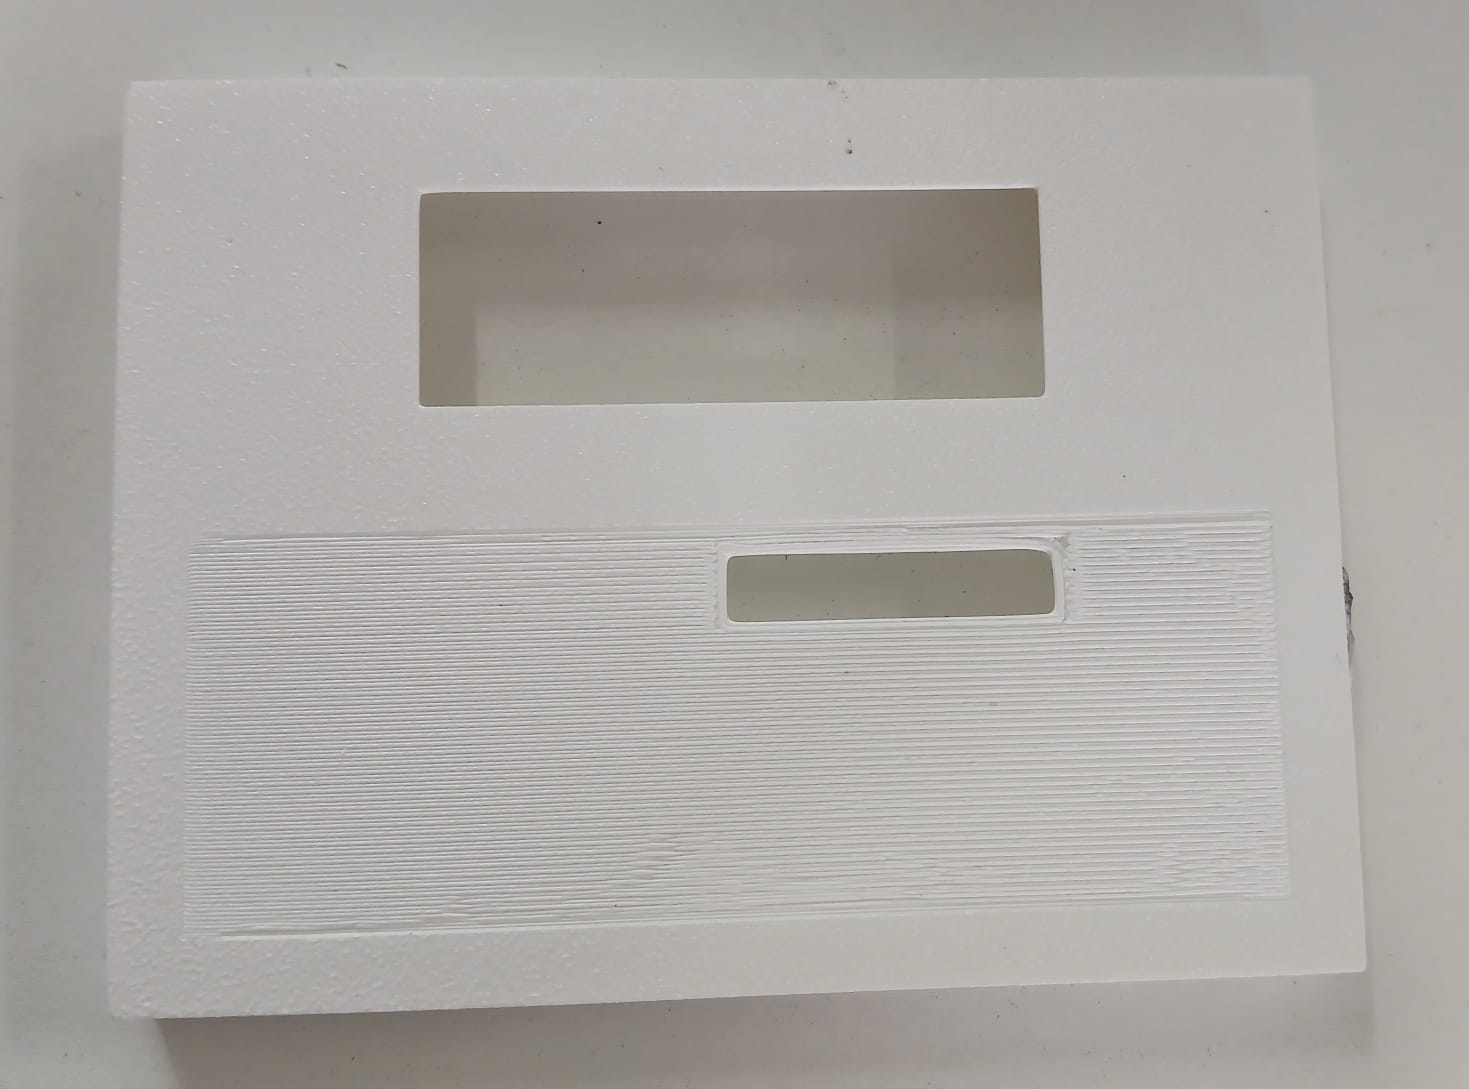
\includegraphics[width=0.45\textwidth]{toplid.jpeg}
    \hfill
    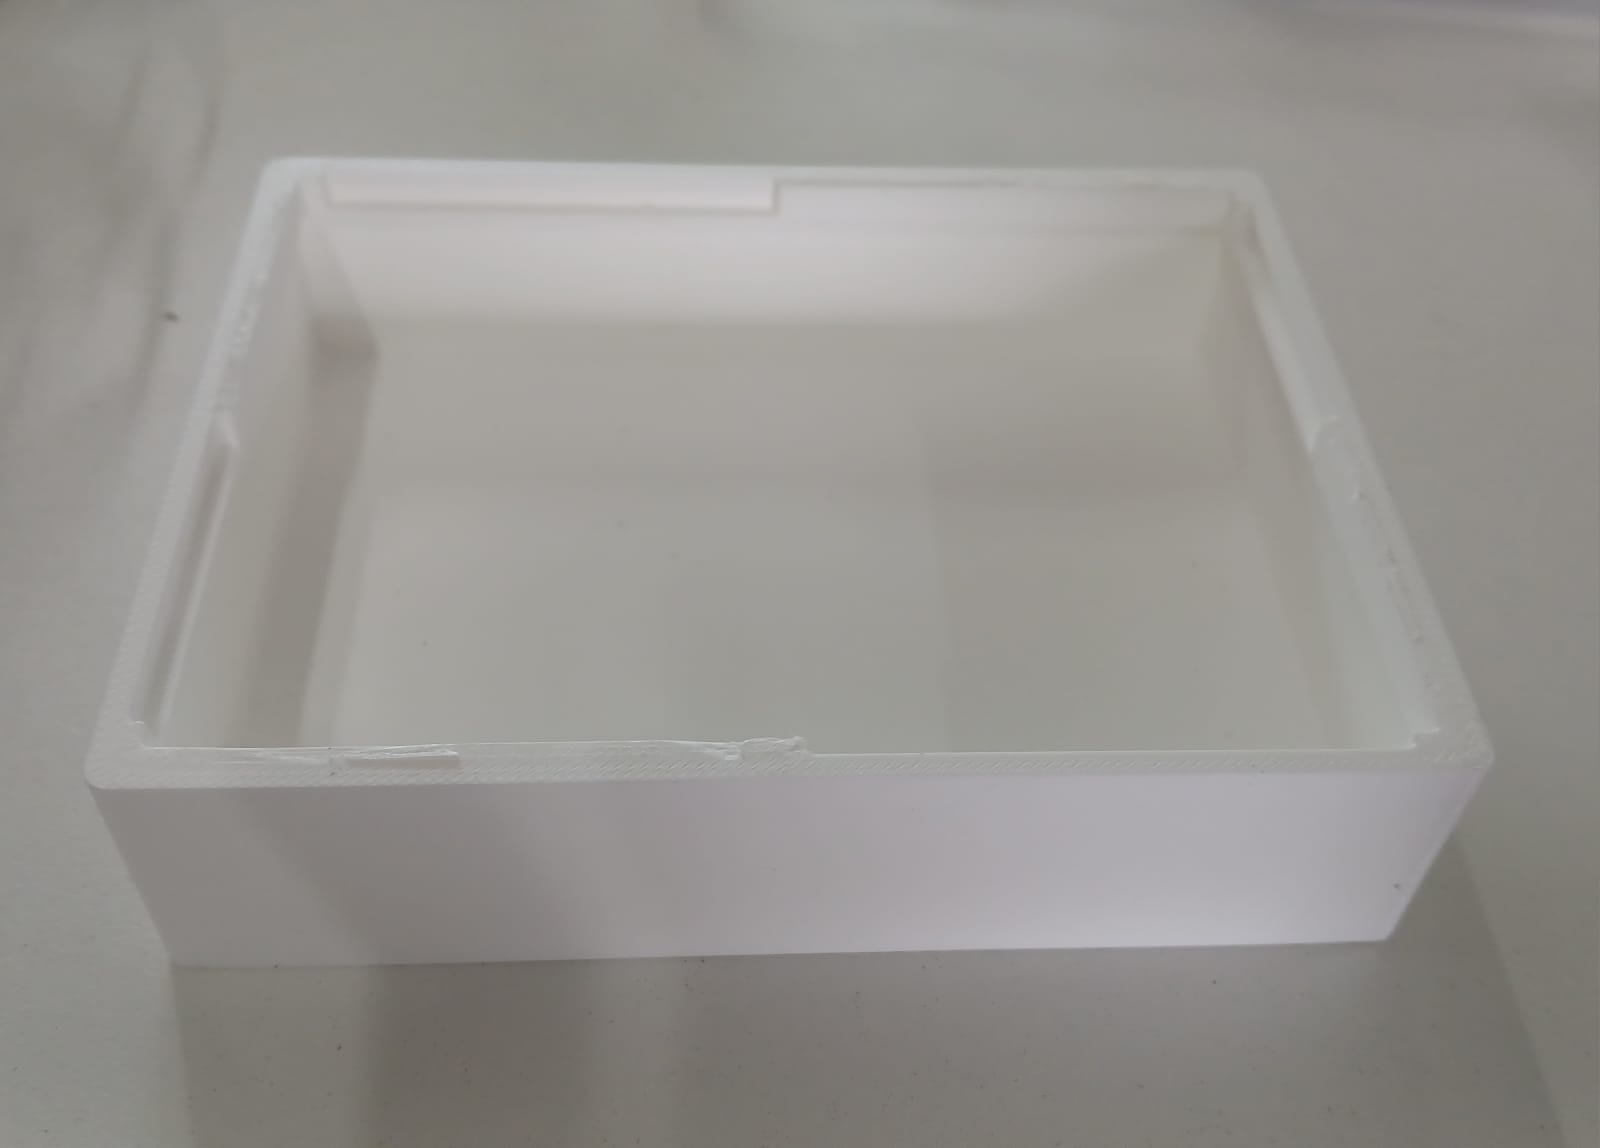
\includegraphics[width=0.45\textwidth]{bottomcase.jpeg}

    \caption{Fusion 360 CAD Models of the Enclosure}
\end{figure}

%%%%%%%%%%%%%%%%%%%%%%%%%%%%%%%%%%%%%%%%%%%%%%%%%%
% 3D PRINTING
%%%%%%%%%%%%%%%%%%%%%%%%%%%%%%%%%%%%%%%%%%%%%%%%%%

\section{3D Printed Enclosure}

After completing the CAD design, both enclosure components were fabricated using a 3D printer with PLA filament.

The printed enclosure was carefully inspected to ensure that all openings aligned correctly with the display, LEDs, push buttons, and USB connector. The perfboard assembly was then mounted inside the enclosure and secured in position.

The enclosure protects the electronic circuit from accidental damage while providing the clock with a professional appearance suitable for long-term use.

\begin{figure}[H]
    \centering
    \includegraphics[width=0.75\textwidth]{enclosure.jpeg}
    \caption{Completed 3D Printed Enclosure}
\end{figure}

%%%%%%%%%%%%%%%%%%%%%%%%%%%%%%%%%%%%%%%%%%%%%%%%%%
% FINAL MODEL
%%%%%%%%%%%%%%%%%%%%%%%%%%%%%%%%%%%%%%%%%%%%%%%%%%

\section{Final Working Model}

The assembled digital clock was tested under continuous operation after installation inside the enclosure. The display refreshed smoothly without noticeable flickering due to multiplexing, and all push buttons responded correctly for time adjustment.

The clock successfully maintained accurate time using the external crystal oscillator. The final implementation demonstrated stable operation, compact hardware design, and reliable performance.

\begin{figure}[H]
    \centering
    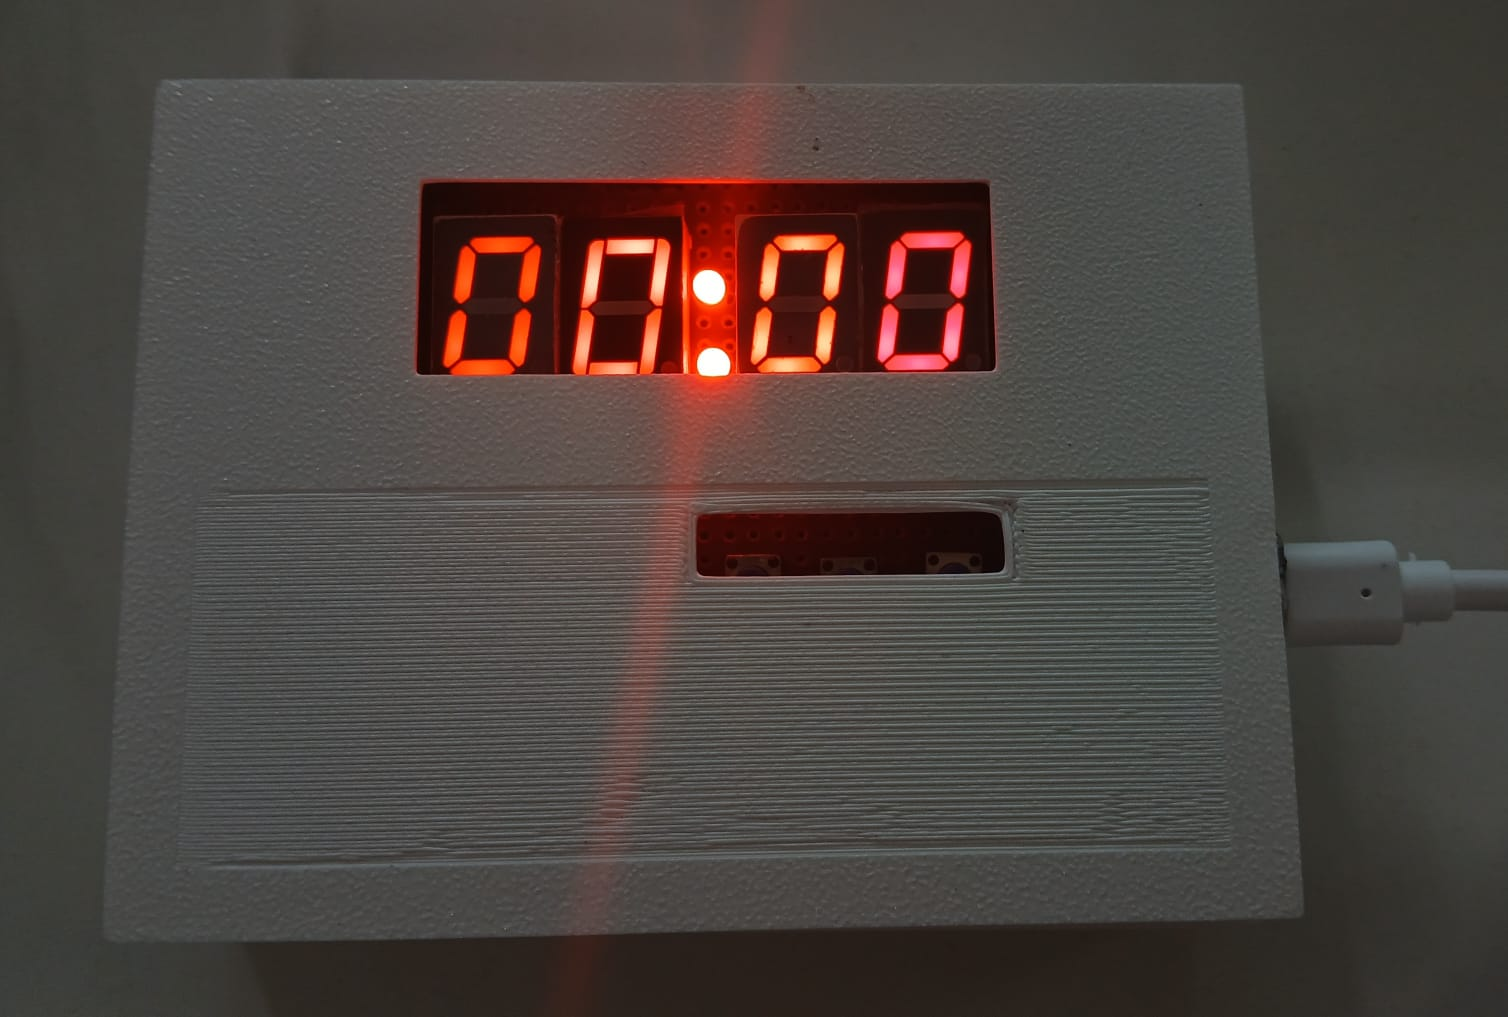
\includegraphics[width=0.75\textwidth]{finalclock.jpeg}
    \caption{Final Working Digital Clock}
\end{figure}

%%%%%%%%%%%%%%%%%%%%%%%%%%%%%%%%%%%%%%%%%%%%%%%%%%
% APPLICATIONS
%%%%%%%%%%%%%%%%%%%%%%%%%%%%%%%%%%%%%%%%%%%%%%%%%%

\section{Applications}

The developed digital clock can be used in several practical applications, including:

\begin{itemize}

\item Desktop digital clocks.

\item Educational embedded systems laboratories.

\item Electronics and microcontroller demonstrations.

\item DIY embedded system projects.

\item Real-time display systems.

\item Academic mini-projects.

\end{itemize}

%%%%%%%%%%%%%%%%%%%%%%%%%%%%%%%%%%%%%%%%%%%%%%%%%%
% ADVANTAGES
%%%%%%%%%%%%%%%%%%%%%%%%%%%%%%%%%%%%%%%%%%%%%%%%%%

\section{Advantages}

\begin{itemize}

\item Compact standalone embedded system.

\item Low power consumption.

\item Accurate timing using crystal oscillator.

\item Easy user interaction through push buttons.

\item Expandable firmware for additional features.

\item Custom-designed protective enclosure.

\item Cost-effective implementation.

\item Easy maintenance due to socket-mounted microcontroller.

\end{itemize}

%%%%%%%%%%%%%%%%%%%%%%%%%%%%%%%%%%%%%%%%%%%%%%%%%%
% FUTURE SCOPE
%%%%%%%%%%%%%%%%%%%%%%%%%%%%%%%%%%%%%%%%%%%%%%%%%%

\section{Future Scope}

Several improvements can be incorporated into the current design to enhance its functionality.

\begin{itemize}

\item Addition of seconds display.

\item RTC module for higher accuracy.

\item Alarm functionality.

\item Automatic brightness adjustment.

\item Battery backup during power failure.

\item Bluetooth or Wi-Fi synchronization.

\item Temperature and humidity display.

\item 12-hour and 24-hour display modes.

\end{itemize}

%%%%%%%%%%%%%%%%%%%%%%%%%%%%%%%%%%%%%%%%%%%%%%%%%%
% CONCLUSION
%%%%%%%%%%%%%%%%%%%%%%%%%%%%%%%%%%%%%%%%%%%%%%%%%%

\section{Conclusion}

The Digital Clock project successfully demonstrates the complete development cycle of an embedded system, beginning from circuit prototyping and firmware development to standalone hardware implementation and mechanical enclosure fabrication.

The project provided practical experience in embedded programming, electronic circuit design, soldering techniques, CAD modelling using Fusion 360, and additive manufacturing through 3D printing.

The final system is compact, reliable, and capable of accurately displaying time using a standalone ATmega328P microcontroller. The successful integration of electronics and mechanical design makes the project suitable for both academic learning and real-world embedded system applications.

\end{document}
